\title{Assignment 3 -- CSC 225}
\author{
	Andrew \bf{Hobden} \\
	Student Number: \bf{V00788452}\\
	Instructor: Venkatesh Srinivasan
}
\date{\today}

\documentclass[12pt]{article}
\usepackage{mathtools}
\usepackage{amssymb}
\usepackage{algpseudocode}
\usepackage{algorithm}

\begin{document}
\maketitle

\section{Trees}
In any tree $T$ with $n$ nodes, the distance between two nodes $u$ and $v$ in $T$ is the number of nodes on the path from $u$ to $v$. The diameter of $T$ is the maximum distance between two nodes in $T$. Describe an $O(n)$ running time algorithm to compute the diameter of a tree using level-order traversal (also known as Breadth First Search).

\begin{center}
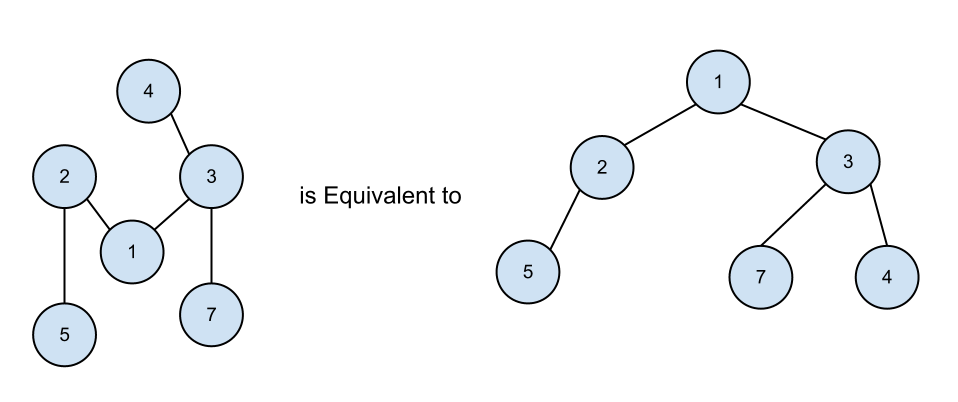
\includegraphics[width=0.6\textwidth]{figures/diameter1.png}
\end{center}
We'll assume the following:
\begin{itemize}
	\item The $root$ of the tree can be any arbitrary node in the tree.
	\item The tree need not be binary.
	\item Each node has a $depth$ attribute we can set.
	\item Each node's children can be found in an array $node$.children
\end{itemize}
\begin{algorithm}
\begin{algorithmic}[1]
	\Function{getFarthestNode}{$T$,$root$}
		\State $toSearch \gets$ new Queue
		\State $depth \gets 0$
		\State $root$.depth($depth$)
		\State $toSearch$.enqeueue($root$)
		\State $farthest \gets root$
		\Comment We want to find the farthest node.
		\While{$toSearch$ is not empty}
			\State $cur \gets toSearch$.dequeue()
			\State $depth \gets depth+1$
			\For{Each $child$ in $cur$.children}
				\State $child$.depth($depth$)
				\State $toSearch$.enqueue($child$)
				\If{$farthest.depth > child.depth $}
					\State $farthest \gets child$
					\Comment This is the new farthest node.
				\EndIf
			\EndFor
		\EndWhile
	\State \Return $farthest$
	\Comment The node farthest from the given root.
	\EndFunction
	\Function{diameter}{$T$, $root$}
		\State $farthest \gets$ getFarthestNode($T$, $root$)
		\Comment Get the farthest node
		\State $target \gets$ getFarthestNode($T$, $farthest$)
		\Comment Farthest from that
		\State \Return $target$.depth
		\Comment This is the diameter
	\EndFunction
\end{algorithmic}
\end{algorithm}
Perhaps this requires some justification... Consider the example tree:
\begin{center}
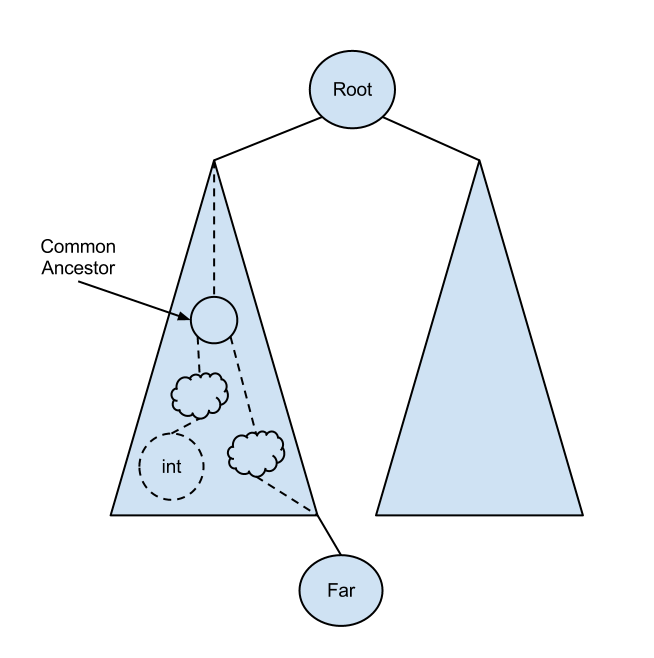
\includegraphics[width=0.8\textwidth]{figures/diameter2.png}
\end{center}
Lets suppose $far$ is our node at maximum depth, and that $int$ is some node within the subtree which is claimed to have a longer path. Given that $far$ and $int$ do not have the same depth, $far$ must have a greater depth. Since $far$ and $int$ share a common ancestor, $far$ by definition is farther away then $int$ from the other side of the claimed longer path.


\section{Heap Sort}
Illustrate the performance of heap-sort algorithm on the following input sequence: $[2,5,16,4,10,23]$. \\
\subsection{Heapifying}
\begin{center}
\includegraphics[width=0.8\textwidth]{figures/heapsort.jpg}
\end{center}
\subsection{Removing}
\begin{center}
\includegraphics[width=0.8\textwidth]{figures/heapsort2.jpg}
\end{center}
\subsection{Performance}
The overall performance of this algorithm should be $ O(n log(n) )$

\section{Priority Queues}
Prove that it is impossible to develop a comparison-based implementation of the Priority Queue ADT in which both insert and removeMin methods guarantee to use O(log log n) comparisons in the worst case.
We will assume that the priority queue can be {\bf considered} a min heap (though it is not neccessarily so) where:
\begin{itemize}
	\item Each node stores a distinct number in $S$, called its key.
	\item Each node's key is always greater then its parents
\end{itemize}
Therefore, to $insert()$ we will need to perform a series of comparisons to ensure the new node is placed appropriately within the 'heap'. %TODO
To $removeMin()$ we can use an $O(log(n))$ operation of pulling off our 'heap's root and bubbling as neccessary. \\
Therefore we will attempt to prove that, in a comparison based implementation following from the above, that $insert()$ requires $>O(log(log(n)))$ time.
\subsection{Operation Lower Bounds Method}
Consider our heap, it has a height of $\lfloor log(n) \rfloor$. This means, in the worst case, we will need to do $\lfloor log(n) \rfloor$ comparisons for an element to be placed at the bottom of the heap. Since $\lfloor log(n) \rfloor > log(log(n))$, our proof is complete for $insert()$. \\
We do not need to prove anything for $removeMin()$ since we only needed to show that one of the conditions is untrue, and both would be required to be true for it to be possible. However it can be followed from a standard $removeMin()$ on a heap, which is known to be $O(log(n))$.
\subsection{Comparison Sorting Bounds Method}
Using the lower bounds of comparison sorting, $O(n*log(n))$, we can demonstrate that this priority queue is not possible.\\ First, we'll note that Heapsort (Or {\bf Priority Queue Sort}) has a worst case running time of $O(n*log(n))$.\\
Second, we'll assume that the Priority queue described above {\bf is} possible, and insert our elements to be sorted into the queue (Each in $O(log log n)$ time). Then, we will perform repeated $removeMin()$ calls, each with $O(log log n)$ time. \\
The resulting sort's time complexity is not compatible with the proven bounds of comparison sorting. Therefore the Priority Queue described is impossible.

\section{Sorting}
Suppose that we are given a sequence $S$ of $n$ elements, each of which is an integer in the range $[0,n^2-1]$. Describe a simple algorithm to sort $S$ in $O(n)$ time.
\linebreak
\linebreak
We will have $n$ elements between $0...n^2-1$. Since $n^2-1$ will in general have (much) less then $n$ digits, we'll then use a bucket sort with buckets representing one of the integer values between $0-9$. Since this means we will have less then $n$ sets of 10 buckets, we will be within $O(n)$ space complexity.
\paragraph{Assumptions}
\begin{itemize}
	\item 12 == 012 == 0012 == 00012 == ...
	\item $k$ is the digit we are sorting.
\end{itemize}
\begin{center}
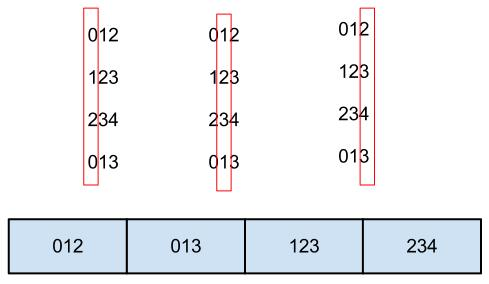
\includegraphics[width=0.8\textwidth]{figures/bubblesort.jpg}
\end{center}
\clearpage
\begin{algorithm}
\begin{algorithmic}[1]
	\Function{bucketsort}{array, k}
		\If{k is 0}
			\State \Return array
			\Comment Return early, we're already done.
		\EndIf
		\State buckets $\gets$ new array of $10$ (empty) lists
		\For{$i \gets 0$ to $length(array)-1$}
			\State slot $\gets$ $k^{th}$ most signifigant digit of array[i]
			\State buckets[slot] $\gets$ array[i]
		\EndFor
		\For{bucket in buckets}
			\State bucketsort(bucket, k-1)
			\Comment Sort via the 2nd MSD
		\EndFor
		\State \Return Concatenation of buckets
		\Comment Using this term loosely.
	\EndFunction
\end{algorithmic}
\end{algorithm} %TODO

\section{Hashing}
Show that the expected search time for hashing using open addressing is at most $\frac{1}{1- w}$ where $w$ is the load factor. State your assumption.

\subsection{Assumption}
Each key is equally likely to have any one of the $ t! $ permutations as it's probe sequence, independent of the other keys. (Uniform hashing)
Furthermore, we'll assume that $ w = \frac{n}{t} $ where $n$ is the number of items and $t$ is the number of slots.

\subsection{Proof}
We'll note the following:
\begin{itemize}
	\item 1 probe is always needed.
	\item Probability 2 probes are needed: $\frac{n}{t}$
	\item Probability 3 probes are needed: $\frac{n}{t}*\frac{n-1}{t-1}$
	\item Probability 4 probes are needed: $\frac{n}{t}*\frac{n-1}{t-1}*\frac{n-2}{t-2}$
\end{itemize}
From statistics we can note:
\begin{displaymath}
	E[X]=\sum_x xP_x[X=x]
\end{displaymath}
\begin{displaymath}
	E[X]=\sum_x Pr[X\geq x]
\end{displaymath}
From above:
\begin{itemize}
	\item $Pr[x \geq 1] = 1$
	\item $Pr[x \geq 2] = \frac{n}{t}$
	\item $Pr[x \geq 3] = \frac{n}{t}*\frac{n-1}{t-1}$
\end{itemize}
Therefore we find that
\begin{displaymath}
	E[X]=1+\frac{n}{t}+\frac{n}{t}\frac{n-1}{t-1}+...
\end{displaymath}
We'll approximate $ \frac{n-i}{t-i} = \alpha = w $, this is justified since $ \frac{n-i}{t-i} < \frac{n}{t}$
\begin{displaymath}
	E[X] \leq 1 + w + w^2 + ...
\end{displaymath}
Which is equivalent to $ E[X] \leq \frac{1}{1-w} $

\section{Hashing 2}
How will you preform deletion from a hash table that uses linear probing to resolve collisions if you are not allowed to use a special marker to represent deleted elements?


Without having a special marker to represent the deleted elements we would have two viable options.
One would be to keep a seperate array containing the locations of deleted elements, and when stepping through to check to make sure elements are not deleted. However this seems to be going against the idea of the question.

The second way would be to, perform the following steps:
\begin{enumerate}
	\item Find the desired element to be removed.
	\item Remove it.
	\item Move to the next slot to be checked.
	\item If there is something in this slot remove it, then re-add it.
	\item Repeat from step 3 until you hit an empty slot.
\end{enumerate} 
Or, as loose pseudocode
\begin{algorithm}
\begin{algorithmic}[1]
	\Function{remove}{$n$, $step$}
		\State $slot$ $\gets$ Hash($n$)
		\State Remove Table($slot$)
		\Repeat
			\State $slot \gets slot+step$
			\If{Table($slot$) is not empty}
				\State $element \gets$ Remove Table($slot$)
				\State Re-add $element$
			\EndIf
		\Until{Table($slot+step$) is empty}
	\EndFunction
\end{algorithmic}
\end{algorithm}
\end{document}